\section{Ergebnisse}
\subsection{Npoint-Scan der Sonne}
Der npoint Scan ergab, dass das Intensitätsmaximum der Sonne einen Offset zur in der Katalogdatei für die Sonne eingetragenen Position aufwies. Abbildung %\ref{npoint_sun} zeigt einen Plot des npoint Scans.
Die Auswertung des Cross-Scans zeigte, dass das Maximum des Elevationsscans um 3241,6 niedriger ausfiel als das Maximum des Azimutscans. Die Position des Maximums war an der durch den npoint Scan ermittelten Stelle.

\subsection{Cross-Scan der Sonne}
bla bla (wie daten entstanden, wie fehlerbalken entstanden)

\begin{figure}
		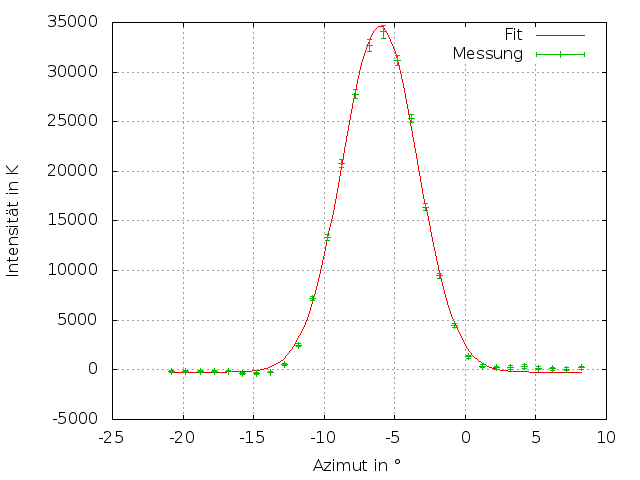
\includegraphics[width=.9\textwidth]{images/sun_azimut}
\caption{ Plot der Intensität der Sonne in Abhängigkeit des Azimutwinkels }
\label{fig:sunaz}
\end{figure}

\begin{figure}
		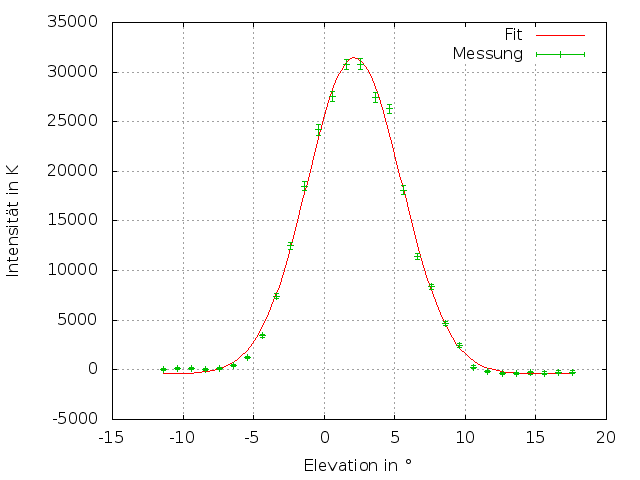
\includegraphics[width=.9\textwidth]{images/sun_elevation}
\caption{ Plot der Intensität der Sonne in Abhängigkeit des Elevationswinkels }
\label{fig:sunel}
\end{figure}

\subsection{Bestimmung der Halbwertsbreite der Antennenkeule}
Zur Bestimmung der Halbwertsbreite der Antennenkeule wurden die Messdaten mit einer Gauß-Funktion gefittet (siehe Abb. \ref{fig:sunaz} und \ref{fig:sunel}). Für die Funktion

\begin{equation}
f(x) = a \cdot e^{- \frac{(x-d)^2}{b}} + c
\label{form:FWHMfit}
\end{equation}

ergaben sich dabei Werte, wie in Tabelle \ref{tab:FWHM} zu sehen.

\begin{table}
\centering
\begin{tabular}{ccc}
Parameter	&			Wert der Azimutmessung	&	Wert der Elevationsmessung \\
\midrule
a			&			34861 $\pm$ 274			&	31855 $\pm$ 393 \\
b			&			14.32 $\pm$ 0.29		&	22.29 $\pm$ 0.72 \\
c			&			-226.4 $\pm$ 117.0		&	-401.9 $\pm$ 207.3 \\
d			&			-6.045 $\pm$ 0.023		&	2.146 $\pm$ 0.045
\end{tabular}
\caption{Werte des Fits für die Parameter aus \eqref{form:FWHMfit}}
\label{tab:FWHM}
\end{table}

Bei dieser Gauß-Funktion ergibt sich die Halbwertsbreite H folgendermaßen:

\begin{equation}
H = 2 \sqrt{2 \ln 2} \cdot \sqrt{\frac{b}{2}}
\end{equation}

Durch Fehlerfortpflanzung ergibt sich:

\begin{equation}
\delta H = \frac{\sqrt{2 \ln 2}t}{2} \sqrt{\frac{2}{b}} \cdot \delta b
\label{form:FehlerFWHM}
\end{equation}

Aus \eqref{form:FehlerFWHM} ergibt sich dann:

\begin{align*}
H_{\mr{Azimut}} = 6.300\,^\circ \ &\mathrm{und} \ \delta H_{\mr{Azimut}} = 0.062\,^\circ \\
H_{\mr{Elevation}} = 6.545\,^\circ \ &\mathrm{und} \ \delta H_{\mr{Elevation}} = 0.106\,^\circ
\end{align*}

Zusammenfassend ergibt sich also:

\begin{align}
H_{\mr{Azimut}} = 6.30\,^\circ \pm 0.07\,^\circ \\
H_{\mr{Elevation}} = 6.54\,^\circ \pm 0.11\,^\circ
\end{align}

Aufgrund der Rotationssymmetrie der Antennenkeulen, lässt sich die Halbwertsbreite der Keulen durch Mittelwertbildung bestimmen. Dabei folgt aus $ H = \left(H_{\mr{Azimut}} + H_{\mr{Elevation}}\right)/2 $ mittels Fehlerfortpflanzung:

\begin{equation}
\delta H = \frac{\sqrt{{\delta H_{\mr{Azimut}}}^2 + {\delta H_{\mr{Elevation}}}^2}}{2}
\end{equation}

Daraus erhält man:

\begin{equation}
H = 6.4226\,^\circ \pm 0.0616\,^\circ \approx 6.42\,^\circ \pm 0.07\,^\circ
\end{equation}